\documentclass[conference]{IEEEtran}
\usepackage{amsmath,amssymb}
\usepackage{graphicx}
\usepackage{booktabs}
\usepackage{multirow}
\usepackage{url}

\title{Physics-informed AI for Fast Three-phase N-1 Security Screening in Unbalanced Microgrids}
\author{Student Name, Advisor Name}

\begin{document}
\maketitle

\begin{abstract}
This mini-paper studies fast static N-1 security screening for unbalanced microgrids. A pandapower-based three-phase power-flow pipeline is used to generate post-contingency labels under voltage, loading, voltage-unbalance, service-loss, and convergence criteria. Several screening models are compared, including traditional ML baselines, a physics-informed multi-task MLP, and a phase-aware GNN. The goal is not to replace three-phase power flow, but to prioritize high-risk contingencies while maintaining high recall.
\end{abstract}

\section{Introduction}
Unbalanced microgrids and low-voltage feeders can experience phase-specific voltage, current, and unbalance violations under component outages. Exhaustive three-phase N-1 scans are accurate but expensive when many operating scenarios and contingencies must be assessed. This work evaluates AI-based pre-screening models for fast high-recall contingency prioritization.

\textbf{Contributions:}
\begin{itemize}
    \item A reproducible three-phase N-1 labeling workflow for microgrid security screening.
    \item A phase-aware violation definition including voltage, loading, VUF, service-loss, and non-convergence labels.
    \item A comparison of engineering rules, ML baselines, PI-MLP, and phase-aware GNN models under high-recall screening metrics.
    \item A validation suite for dataset lineage, no-leakage feature design, metric consistency, and graph invariance checks.
\end{itemize}

\section{Three-phase Microgrid Security Formulation}
For each base-case scenario $x_t$ and contingency $c\in\mathcal{C}$, the target is a binary label $y_{t,c}$ and severity score $s_{t,c}$. The post-contingency quantities include phase voltages $V_{i,\phi}^{c}$, line currents $I_{\ell,\phi}^{c}$, and voltage unbalance factors.

\subsection{Violation Labels}
The final label is the logical OR of low-voltage, high-voltage, loading, VUF, service-loss, critical service-loss, and non-convergence flags.

\section{Dataset Generation}
The dataset is generated using a microgrid-like teaching feeder. Scenario generation controls load level, phase imbalance, PV penetration, and BESS charging/discharging setpoints. Each scenario is combined with a contingency catalog including line outages, PV trips, BESS trip, and PCC outage.

\begin{table*}[t]
\centering
\caption{Dataset statistics for the teaching microgrid N-1 benchmark.}
\label{tab:dataset}
\resizebox{\textwidth}{!}{%
\begin{tabular}{lrrrrrrrrr}
\toprule
dataset & n\_scenarios & n\_contingencies & expected\_samples & actual\_samples & safe\_samples & unsafe\_samples & power\_flow\_solved\_rows & service\_loss\_skipped\_rows & no\_slack\_skipped\_rows \\
\midrule
Three-phase microgrid N-1 dataset & 7 & 11 & 77 & 77 & 30 & 47 & 35 & 35 & 7 \\
\bottomrule
\end{tabular}
}
\end{table*}


\section{Screening Models}
\subsection{Traditional ML Baselines}
Engineering rules, logistic regression, random forest, gradient boosting, and MLP baselines are trained using no-leakage base-case features.

\subsection{Physics-informed MLP}
The PI-MLP predicts a violation probability, severity score, and component margins. The loss combines classification, severity, component-margin, component-severity consistency, probability-severity consistency, and ranking terms.

\subsection{Phase-aware GNN}
The GNN uses bus-level phase-channel node features, line edge features, and contingency masks to produce a graph-level risk score.

\section{Experiments}
\begin{table*}[t]
\centering
\caption{Holdout comparison of security screening models.}
\label{tab:model_comparison}
\resizebox{\textwidth}{!}{%
\begin{tabular}{llrrrrrrr}
\toprule
stage & model & recall & precision & fnr & pf\_calls\_saved\_fraction & missed\_violations & auprc & auroc \\
\midrule
Week 5 ML baseline & GradientBoosting & 1.000 & 1.000 & 0.000 & 0.400 & 0 & 1.000 & 1.000 \\
Week 6 PI-MLP & PI-MLP full & 1.000 & 1.000 & 0.000 & 0.400 & 0 & 1.000 & 1.000 \\
Week 7 GNN & FlattenedMLP & 1.000 & 1.000 & 0.000 & 0.400 & 0 & 1.000 & 1.000 \\
Week 5 ML baseline & EngineeringRule & 1.000 & 0.857 & 0.000 & 0.300 & 0 & 0.910 & 0.906 \\
Week 6 PI-MLP & BaselineMLP & 1.000 & 0.857 & 0.000 & 0.300 & 0 & 1.000 & 1.000 \\
Week 5 ML baseline & AllUnsafe & 1.000 & 0.600 & 0.000 & 0.000 & 0 & 0.600 & 0.500 \\
Week 5 ML baseline & MLP & 1.000 & 0.600 & 0.000 & 0.000 & 0 & 0.533 & 0.240 \\
Week 5 ML baseline & LogisticRegression & 0.833 & 1.000 & 0.167 & 0.500 & 2 & 1.000 & 1.000 \\
Week 5 ML baseline & RandomForest & 0.833 & 0.909 & 0.167 & 0.450 & 2 & 0.956 & 0.938 \\
Week 7 GNN & PhaseAwareGNN & 0.583 & 0.875 & 0.417 & 0.600 & 5 & 0.913 & 0.875 \\
\bottomrule
\end{tabular}
}
\end{table*}

\begin{table}
\caption{Group-based cross-validation for unseen scenarios and contingencies.}
\label{tab:group_cv}
\begin{tabular}{lllrrrrrr}
\toprule
stage & model & cv_type & folds & mean_recall & mean_fnr & mean_pf_calls_saved & mean_auprc & missed_violations_sum \\
\midrule
Week 5 ML baseline & EngineeringRule & scenario\_group & 3 & 1.000 & 0.000 & 0.323 & 0.912 & 0.000 \\
Week 5 ML baseline & AllUnsafe & scenario\_group & 3 & 1.000 & 0.000 & 0.000 & 0.596 & 0.000 \\
Week 5 ML baseline & LogisticRegression & scenario\_group & 3 & 0.928 & 0.072 & 0.439 & 0.990 & 5.000 \\
Week 5 ML baseline & RandomForest & scenario\_group & 3 & 0.899 & 0.101 & 0.475 & 0.990 & 7.000 \\
Week 5 ML baseline & EngineeringRule & contingency\_group & 3 & 1.000 & 0.000 & 0.310 & 0.971 & 0.000 \\
Week 5 ML baseline & AllUnsafe & contingency\_group & 3 & 1.000 & 0.000 & 0.000 & 0.619 & 0.000 \\
Week 5 ML baseline & RandomForest & contingency\_group & 3 & 0.400 & 0.600 & 0.690 & 0.861 & 28.000 \\
Week 5 ML baseline & LogisticRegression & contingency\_group & 3 & 0.254 & 0.746 & 0.786 & 0.909 & 35.000 \\
Week 6 PI-MLP & PI-MLP full & contingency\_group & 3 & 0.760 & 0.240 & 0.413 & 0.877 & NaN \\
Week 6 PI-MLP & PI-MLP full & scenario\_group & 3 & 0.928 & 0.072 & 0.207 & 0.942 & NaN \\
Week 7 GNN & PhaseAwareGNN & contingency\_group & 11 & 0.896 & 0.104 & 0.247 & NaN & 8.000 \\
Week 7 GNN & PhaseAwareGNN & scenario\_group & 7 & 0.690 & 0.310 & 0.468 & NaN & 18.000 \\
\bottomrule
\end{tabular}
\end{table}

\begin{table}
\caption{Loss ablation for physics-informed MLP training.}
\label{tab:ablation}
\begin{tabular}{rrrrrrrrrrrrlr}
\toprule
threshold & TP & FP & TN & FN & recall & precision & fnr & pf_calls_saved_fraction & missed_violations & auprc & auroc & model & selected_threshold \\
\midrule
0.010 & 12 & 2 & 6 & 0 & 1.000 & 0.857 & 0.000 & 0.300 & 0 & 1.000 & 1.000 & BaselineMLP & 0.010 \\
0.005 & 12 & 1 & 7 & 0 & 1.000 & 0.923 & 0.000 & 0.350 & 0 & 1.000 & 1.000 & PI-MLP no-rank & 0.005 \\
0.005 & 12 & 0 & 8 & 0 & 1.000 & 1.000 & 0.000 & 0.400 & 0 & 1.000 & 1.000 & PI-MLP full & 0.005 \\
\bottomrule
\end{tabular}
\end{table}


\begin{figure}[t]
    \centering
    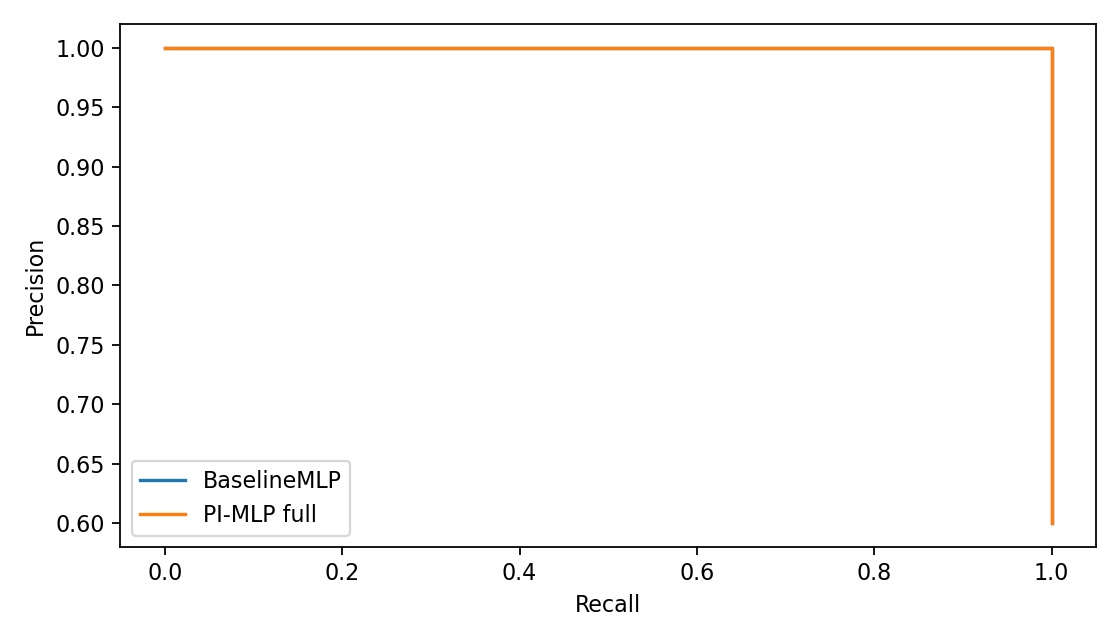
\includegraphics[width=0.95\linewidth]{figures/fig3_week6_precision_recall_curves.png}
    \caption{Precision-recall curves for screening models.}
    \label{fig:pr}
\end{figure}

\begin{figure}[t]
    \centering
    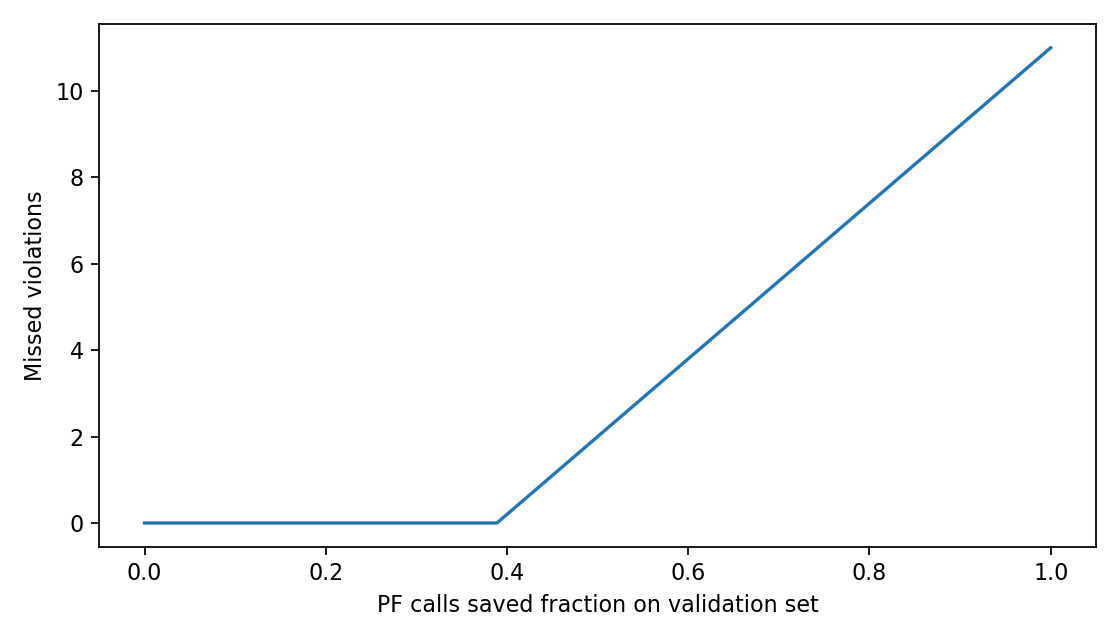
\includegraphics[width=0.95\linewidth]{figures/fig4_week6_saved_calls_vs_missed_violations.png}
    \caption{Tradeoff between saved three-phase power-flow calls and missed violations.}
    \label{fig:saved_calls}
\end{figure}

\begin{figure}[t]
    \centering
    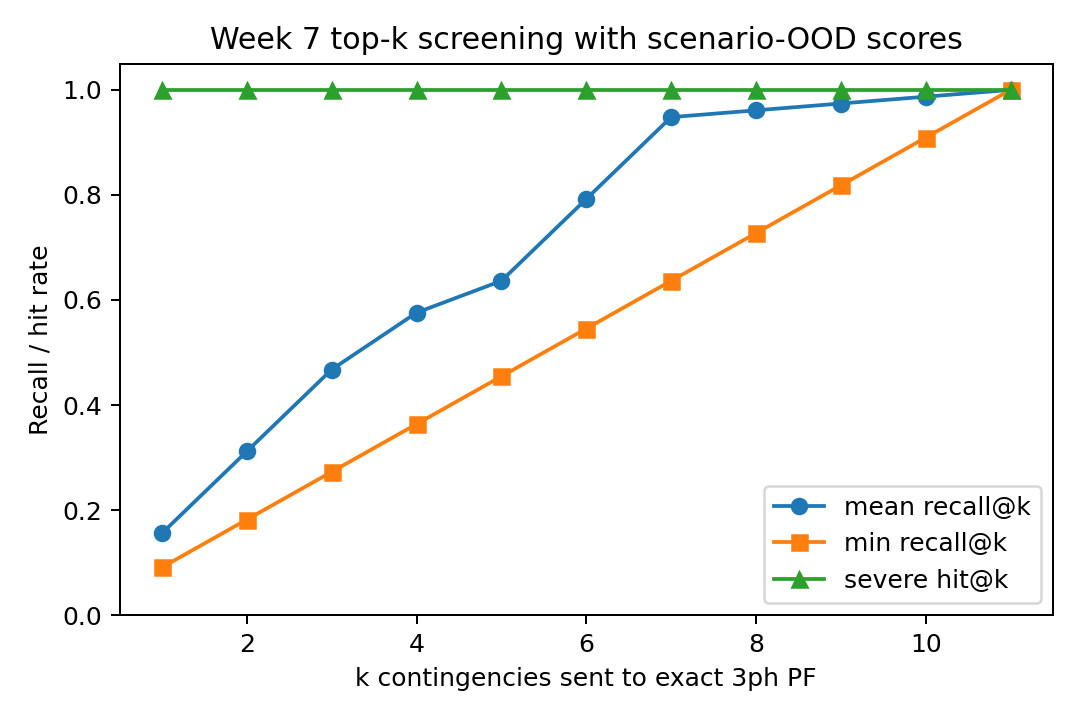
\includegraphics[width=0.95\linewidth]{figures/fig5_week7_topk_violation_recall.png}
    \caption{Top-$k$ violation recall for contingency prioritization.}
    \label{fig:topk}
\end{figure}

\section{Discussion and Limitations}
The current benchmark is intentionally small and teaching-oriented. It supports methodological development and validation logic, but broader claims require additional feeders, stochastic scenarios, islanded-mode modeling, grid-forming inverter models, and real microgrid data.

\section{Conclusion}
This project demonstrates a reproducible workflow for three-phase microgrid N-1 security screening with AI. The main lesson is that high-recall screening, validation discipline, and no-leakage feature design are as important as model architecture.

\end{document}
